% =====================================================================
%  Verified Mechanisms -- Research Engineer take-home
%  Writeup (Part One + Part Two). Graded artifact: this PDF.
%  Body: 1-10 pages; appendix unlimited.
%
%  Draft v2 -- modular. Each chapter lives in sections/*.tex.
%  Compile:  tectonic -X compile main.tex
% =====================================================================
\documentclass[11pt]{article}

% ---- encoding / fonts ----
\usepackage[T1]{fontenc}
\usepackage[utf8]{inputenc}
\usepackage{lmodern}
\usepackage{microtype}

% ---- layout ----
\usepackage[margin=1in]{geometry}
\usepackage{enumitem}
\setlist{nosep,leftmargin=1.4em}
\setlength{\parskip}{0.38em}
\setlength{\parindent}{0pt}
\setlength{\emergencystretch}{2em}

% ---- math ----
\usepackage{amsmath,amssymb}

% ---- tables / figures ----
\usepackage{booktabs}
\usepackage{tabularx}
\usepackage{array}
\usepackage{graphicx}
\usepackage{caption}
\captionsetup{font=small,labelfont=bf}

% ---- color / links ----
\usepackage{xcolor}
\definecolor{linknavy}{RGB}{20,55,110}
\usepackage[colorlinks=true,linkcolor=black,urlcolor=linknavy,citecolor=black]{hyperref}
\hypersetup{
  pdftitle={Lean as the Coordination Signal},
  pdfauthor={Ayrton Porto}
}

% ---- tikz for the ladder figure ----
\usepackage{tikz}
\usetikzlibrary{arrows.meta,positioning,fit,calc}

% =====================================================================
%  Notation macros -- keep arm names consistent everywhere
% =====================================================================
\newcommand{\SQ}{\textsf{S-Q}}     % Qwen solo
\newcommand{\SG}{\textsf{S-G}}     % GPT-OSS solo
\newcommand{\RQ}{\textsf{R-Q}}     % Qwen self-repair
\newcommand{\RG}{\textsf{R-G}}     % GPT-OSS self-repair
\newcommand{\HQG}{\textsf{H-QG}}   % handoff Qwen -> GPT
\newcommand{\HGQ}{\textsf{H-GQ}}   % handoff GPT -> Qwen
\newcommand{\Uni}{\textsf{U}}      % derived solo union
\newcommand{\Sdev}{\textsf{S\_dev}}
\newcommand{\Seval}{\textsf{S\_eval}}
\newcommand{\qwen}{\texttt{qwen3.5-flash}}
\newcommand{\gptoss}{\texttt{gpt-oss-120b}}
\newcommand{\pass}{\textsc{pass}}
\newcommand{\fail}{\textsc{fail}}

% =====================================================================
\title{\bfseries Lean as the Coordination Signal:\\[0.2em]
\large A Finite Repair Ladder for Qwen\,$+$\,GPT-OSS Proof Search}
\author{Ayrton Porto\\
\small Research Engineer take-home --- Verified Mechanisms}
\date{2 September 2026}

\begin{document}
\maketitle

% ---------------------------------------------------------------------
%  Abstract -- honest causal framing: portfolio+repair beats solos;
%  cross-model handoff is a studied negative result.
% ---------------------------------------------------------------------
\begin{abstract}
\noindent
I make two fixed chat models --- \nolinkurl{qwen/qwen3.5-flash-02-23} and
\nolinkurl{openai/gpt-oss-120b} --- cooperate to produce Lean~4 proofs, and I
report honestly on \emph{which} form of cooperation actually pays. The design
principle is that \emph{Lean is a coordination signal at every step, not only the
final judge}: each candidate is compiled, its structured diagnostics drive a
repair, and any cross-model handoff is seeded with the exact compiler message
rather than free prose. The mechanism is a small, finite escalation ladder ---
free tactics, then same-model repair, then a seeded handoff, then a combining
fallback --- that returns on the first accepted proof. Every reported number is
\emph{substantive}: it survives an anti-tautology guard that rejects the circular
``restate-the-answer'' proofs a permissive checker accepts. On the frozen
nine-problem development set the integrated policy scores \textbf{5/9 substantive},
against \textbf{3/9} for each vanilla solo model and \textbf{4/9} for their union.
The controlled solo/repair/handoff matrix locates the cause: the added points come
from \emph{structured same-model repair and portfolio routing over complementary
strengths}, not from cross-model handoff. Indeed my clearest Part~Two finding is
\emph{negative} and useful: handing one model's proof to the other for repair
added no win and, in one case, destroyed a proof a single model would have found
alone. Verification and routing --- not model-versus-model debate --- are the
mechanism the data support. Beyond the reliable core, the system reaches a genuine
IMO multi-theorem problem through test-time sampling scale (probabilistically, not
reliably), and I characterize precisely where the frontier stops: a residual stage
mints and reuses \emph{verified} lemmas but does not always assemble the hard goal.
I treat the study as exploratory ($n=9$, stochastic models) and report per-problem
outcomes, a failure taxonomy, transcripts, a spend ledger, and a holdout estimate.
\end{abstract}

% ---------------------------------------------------------------------
%  1. Introduction & task
% ---------------------------------------------------------------------
\section{Introduction}
\label{sec:intro}

\subsection{The task}
The take-home has two graded parts. \textbf{Part~One} asks for a coordination
layer that makes two fixed models --- Qwen (\nolinkurl{qwen/qwen3.5-flash-02-23})
and GPT-OSS (\nolinkurl{openai/gpt-oss-120b}), both via OpenRouter --- solve math
problems and prove the answers in Lean~4. Scoring is mechanical: on a private
holdout of roughly a dozen problems, a problem earns one point iff its Lean file
passes the open-source comparator, and a simple design that can be fully
understood is explicitly preferred over a complex one that scores marginally
better. \textbf{Part~Two} asks the scientific question: does the collaboration
beat either model alone, on which problems, and what does one model contribute
that the other lacks --- reported per problem, with a failure taxonomy, transcript
case studies, confounds, a spend ledger, and a holdout estimate.

I follow the judging conditions stated in the task brief and \texttt{RULES.md}:
\$1 and eight hours of wall-clock per problem, enforced by the grader's runner.
Separately, I used a stricter twenty-minute cap in part of the validation campaign
to test whether the reliable core survives under substantially less compute
(\S\ref{sec:results}). The runtime is narrow: only
\nolinkurl{openrouter.ai} and only the two model IDs; no web tools, no retrieval,
no variants. The Lean container runs offline, and the graded entrypoint is a
single agent module.

\subsection{Approach: from zero, incrementally, against the literature}
I was the sole applicant and began without a preferred architecture to defend
(coding assistants were used for scaffolding and editing, disclosed in
Appendix~\ref{app:llm}). My background was \emph{autoformalization}, not
AI-for-theorem-proving, so the starting point was a blank sheet, and I built from
less to more: start with the cheapest thing that
can work, measure it, and add a mechanism only when failures demand it --- checking
each against what already exists (compiler-in-the-loop repair, draft--sketch--prove,
premise selection, lemma banking) to avoid reinventing it blindly. Two early
observations shaped everything: these models are cheap to call, so sampling and
combining candidates was economical from the start; and Lean's feedback is a better
coordination medium than natural language, because a compiler error is compact,
objective, and model-agnostic, whereas two chat models that ``debate'' in prose
mostly flatter each other.

\subsection{What I found}
Every figure below is \emph{substantive} --- it survives an anti-tautology guard
(\S\ref{sec:mechanism}) --- and I treat the study as exploratory ($n=9$, single
runs of stochastic models).
\begin{itemize}
  \item \textbf{A Lean-gated portfolio clears the solos.} One integrated policy,
        \textbf{5/9} on the development set, against 3/9 for each vanilla solo and
        4/9 for their union (\S\ref{sec:results}).
  \item \textbf{The cause is repair and routing, not cross-model handoff.} The
        added points come from structured same-model repair over complementary
        strengths; handing one model's proof to the other added no win and
        sometimes hurt --- a clean negative result (\S\ref{sec:parttwo}).
  \item \textbf{The frontier is wider than the reliable core.} Across
        configurations the system has verified model-generated proofs for
        \textbf{6/9} development and \textbf{10/16} sample problems, including an
        IMO problem reached by test-time sampling scale --- probabilistically
        (\S\ref{sec:frontier}).
  \item \textbf{It repeats at judge caps.} A full-caps stress run passed the same
        \textbf{9/16} on two independent nights (\S\ref{sec:results}).
\end{itemize}
Source, transcripts, and run artifacts are in the accompanying repository; exact
run identifiers and spend are in Appendix~\ref{app:runs}.

% ---------------------------------------------------------------------
%  2. Mechanism: Lean-gated coordination (Part One design)
% ---------------------------------------------------------------------
\section{Mechanism: Lean-gated coordination}
\label{sec:mechanism}

\subsection{Design principle: Lean at every step, not only at the end}
The comparator judges once. My system uses Lean far more often than that: the
unit of work is a loop, not a single generation.
\[
\text{candidate}
\;\xrightarrow{\text{Lean}}\;
\text{structured diagnostic}
\;\xrightarrow{\text{model}}\;
\text{repair}
\;\xrightarrow{\text{Lean}}\;
\cdots
\]
Every candidate is compiled against a clean Mathlib environment; the service
returns typed messages, a sorry flag, and timing. Those messages --- not a
model's opinion of its own proof --- decide what happens next. The consequence I
rely on throughout: \textbf{cross-model coordination happens over the compiler's
output, never over prose.} When a stuck proof passes from one model to the other,
it carries the failed candidate plus the exact Lean error, and the second model
is asked to repair. There is no natural-language debate between agents, because a
Lean diagnostic is a stronger, cheaper, and more objective signal than one model
critiquing another in English. Three invariants hold at every rung: no sorry or
admit, no new axioms, and no silent rewriting of the theorem statement --- so
that ``Lean accepted it'' means to me what it will mean to the grader.

\subsection{A finite escalation ladder}
The agent is a \emph{finite} ladder. Success returns immediately; on failure the
next rung runs until it stalls, hits its cap, or the ladder is exhausted. The
order is deliberate --- cheapest and most reliable first, most expensive and most
speculative last (Figure~\ref{fig:ladder}):

\begin{enumerate}
  \item \textbf{T0 --- tactic sweep.} Zero-model closing tactics on the locked
        challenge. Free wins on easy goals, no API spend.
  \item \textbf{Same-model repair champions (Qwen, then GPT-OSS).} One model
        proposes, Lean checks, the \emph{same} model repairs from the failed
        proof and the exact messages, under a turn budget.
  \item \textbf{Seeded cross-model handoff.} The best failed Qwen candidate is
        repaired by GPT-OSS, and vice versa --- carrying the Lean context
        forward, not restarting.
  \item \textbf{Independent slot / whole fallback.} Split the file into locked
        declarations, sample and repair each, recombine under a strict integrity
        check. This is where cheap multi-sampling pays off, and where hard
        multi-theorem problems tend to fall.
  \item \textbf{Bounded program/bridge experiment}, then a \textbf{residual
        lemma-banking stage} (\S\ref{sec:frontier}) if wall remains.
  \item \textbf{Stop} --- accept, stall, or exhausted.
\end{enumerate}

The ladder is the design thesis made concrete: it starts from ``less'' (a free
tactic sweep) and escalates to ``more'' only as the problem resists, and it never
averages the two models --- it \emph{routes} between them and lets Lean
adjudicate each step. This routing is exactly what lets one policy collect wins
that are otherwise split across the two models (\S\ref{sec:results}).

\begin{figure}[h]
\centering
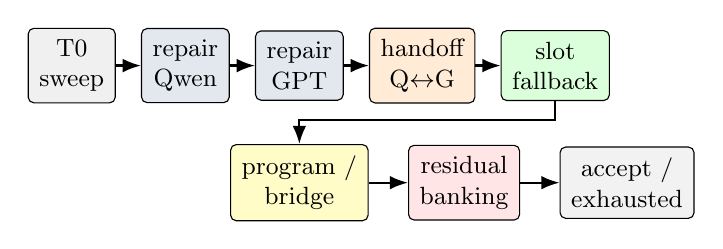
\begin{tikzpicture}[
  font=\small,
  box/.style={draw, rounded corners=2pt, align=center, inner sep=4pt,
              minimum height=0.72cm},
  arr/.style={-{Latex}, thick}
]
\node[box, fill=black!6]   (t0)  {T0\\ sweep};
\node[box, right=0.32cm of t0, fill=linknavy!12] (rq) {repair\\ Qwen};
\node[box, right=0.32cm of rq, fill=linknavy!12] (rg) {repair\\ GPT};
\node[box, right=0.32cm of rg, fill=orange!16]   (h)  {handoff\\ Q$\leftrightarrow$G};
\node[box, right=0.32cm of h,  fill=green!14]    (fb) {slot\\ fallback};
\node[box, below=0.55cm of rg, fill=yellow!22]   (exp){program /\\ bridge};
\node[box, right=0.5cm of exp, fill=red!10]      (res){residual\\ banking};
\node[box, right=0.5cm of res, fill=black!5]     (stop){accept /\\ exhausted};
\draw[arr] (t0) -- (rq);
\draw[arr] (rq) -- (rg);
\draw[arr] (rg) -- (h);
\draw[arr] (h)  -- (fb);
\draw[arr] (fb.south) -- ++(0,-0.24cm) -| (exp.north);
\draw[arr] (exp) -- (res);
\draw[arr] (res) -- (stop);
\end{tikzpicture}
\caption{The finite coordination ladder. Lean accepts or rejects at every rung;
cheap and reliable rungs run first. Residual banking is post-ladder spend, not
the spine.}
\label{fig:ladder}
\end{figure}

\subsection{Acceptance hygiene, and why it is a feature}
A proof accepted by a warm REPL during search is not automatically a proof I
submit. Every final candidate passes a \textbf{strict integrity} guard:
declaration signatures are immutable up to the proof body, answer shapes and
numeric values are checked against the locked problem, and known circular tricks
are rejected. This matters more than it sounds. A model can ``solve'' a Putnam
answer-set problem by \emph{redefining the answer set to be the question} --- for
\texttt{putnam\_2018\_a1}, declaring the solution set to be exactly the pairs
satisfying the left-hand side, so the required equivalence collapses to a
reflexivity and the comparator accepts a proof that establishes nothing. My guard
infers the answer shape from the challenge and rejects such
set-builder / $\lambda$-plus-reflexivity tautologies. I therefore report
\emph{substantive} passes only. Everything counted in this report is a proof of
the actual statement --- a stricter and more defensible bar than raw comparator
acceptance, and the reason my headline numbers hold up when they are re-run.

% ---------------------------------------------------------------------
%  3. Experimental setup
% ---------------------------------------------------------------------
\section{Experimental setup}
\label{sec:setup}

\subsection{Problems and split}
The kit ships sixteen sample problems in the holdout's format. I froze a
development set \Sdev{} ($n=9$) for tuning and an evaluation set \Seval{} ($n=7$),
and report Part~Two science on \Sdev. \Sdev{} spans easy algebra, number-theoretic
identities, and hard olympiad/Putnam statements, so a single number never hides
the difficulty spread.

\subsection{The metric: substantive, not merely accepted}
I track two signals and never conflate them:
\begin{itemize}
  \item \textbf{Comparator pass} --- the Lean file is accepted by the open-source
        comparator. This is the mechanical quantity the grader scores.
  \item \textbf{Substantive} --- the pass also proves the \emph{actual} statement,
        surviving the integrity and anti-tautology guards
        (\S\ref{sec:mechanism}). A pass that only restates the goal does not
        count.
\end{itemize}
\textbf{Every headline number in this report is substantive.} This is a stricter
bar than the task requires, and I adopt it on purpose: it is the only count that
survives an independent re-run with a statement-locked comparator, and it is what
separates a real result from an inflated one.

\subsection{Caps}
The judge enforces \$1 and 8\,h per problem. A few development-matrix runs use
tighter measurement caps so a full sweep fits a small budget; the judge-caps
stress run in \S\ref{sec:results} uses the full \$1/8\,h. Because a repair turn
costs a fraction of a cent, the binding constraint on hard problems was
wall-clock, not the dollar cap --- which is why the ladder can afford a free
sweep, sampled candidates, and a combine step before the expensive residual stage.

\subsection{Part~Two conditions}
To ask whether collaboration beats solo, I hold the code path and caps fixed and
vary only the roles: \SQ/\SG{} (each model solo, on the kit's existing multi-turn
Lean-repair baseline), \RQ/\RG{} (explicit propose/repair, same model), and
\HQG/\HGQ{} (cross-model handoff, each direction). Two points of hygiene. The solo
conditions use the kit's real repair baseline --- I do \emph{not} redefine
``solo'' as a weaker single shot to flatter collaboration. And the \emph{Solo
Union} $\Uni = \SQ \lor \SG$ is \emph{derived}, not a run: it is the natural
non-collaborative baseline any coordination layer must beat to justify itself.

\subsection{Confounds, stated once}
So the results read as prose, the caveats live here: solo baselines sometimes had
more turns than the repair budgets (secondary metrics reported, not perfectly
matched); some matrix cells use measurement caps, not judge caps; with $n=9$ a
one-problem difference is within noise, so I read patterns, not decimals; cells
are single runs of stochastic models; and the full16 stress run is my own sample
suite, not the grader's private holdout.

% ---------------------------------------------------------------------
%  4. Results: the integrated agent (Part One)
% ---------------------------------------------------------------------
\section{Results: a Lean-gated portfolio}
\label{sec:results}

\subsection{The integrated agent on \Sdev}
One policy, one pass, substantive throughout: the ladder scores \textbf{5/9}
(Table~\ref{tab:sdev}). The five wins arrive at three different rungs --- the free
tactic sweep, same-model Qwen repair, and same-model GPT repair --- for about
forty cents total.

\begin{table}[t]
\centering
\caption{Integrated agent on \Sdev, substantive (snapshot). Wins are cheap; the
four hard problems run to \texttt{exhausted}. \texttt{p10}'s closing path is
variable (\S\ref{sec:results}). Total $\approx$\,USD~0.41.}
\label{tab:sdev}
\begin{tabular}{@{}llrr@{}}
\toprule
Problem & Closing rung & Wall (s) & USD \\
\midrule
p01\_linear         & T0 sweep     & 119 & 0.000 \\
p05\_gcd\_mersenne   & T0 sweep     & 105 & 0.000 \\
p03\_sq\_ge\_two\_ab & Qwen repair  & 138 & 0.000 \\
p06\_pow\_mod        & Qwen repair  & 196 & 0.004 \\
p10\_factorial\_pow  & GPT repair   & 387 & 0.009 \\
\midrule
\multicolumn{2}{@{}l}{4 hard problems --- \fail, exhausted}
                     & 2000--3400 & 0.08--0.14 \\
\bottomrule
\end{tabular}
\end{table}

\subsection{It clears the solo baselines --- and where the gain comes from}
On a substantive basis (Table~\ref{tab:matrix}), each vanilla solo model scores
\textbf{3/9} and their union \textbf{4/9}; the integrated policy reaches
\textbf{5/9}. The gain is real but I am precise about its cause. The extra points
are \emph{not} evidence of cross-model collaboration --- they come from two
non-conversational sources: (i) a free tactic sweep that closes easy goals at zero
cost, and (ii) \emph{same-model} repair, which unlocks \texttt{p10} (a problem no
solo configuration solves). Routing between the two models' repair arms captures
their complementary wins in one policy.

I state the honest ceiling of this claim plainly: the union of the two same-model
repair arms, $\RQ\!\lor\!\RG$, also reaches 5/9. So the integrated agent does not
beat an idealized router over those arms; what it adds over such a router is the
free T0 floor and a single, readable control path. The defensible Part~One
statement is therefore \emph{``a finite Lean-gated portfolio of tactics and
same-model repair reaches 5/9, well above the 3/9 solos and 4/9 solo union,''} not
``two models collaborate to beat one.'' A same-budget router over those two arms
remains the right baseline to measure directly (\S\ref{sec:discussion}).

\begin{table}[t]
\centering
\caption{Substantive scores on \Sdev. Raw comparator counts were higher for the
GPT-side arms only because of a Putnam answer-set tautology the guard removes
(\S\ref{sec:mechanism}, Appendix~\ref{app:transcripts}).}
\label{tab:matrix}
\begin{tabular}{@{}lccccccc@{}}
\toprule
\SQ & \SG & \Uni ($\SQ\!\lor\!\SG$) & \RQ & \RG & \HQG & \HGQ & \textbf{Agent} \\
\midrule
3 & 3 & 4 & 4 & 4 & 3 & 2 & \textbf{5} \\
\bottomrule
\end{tabular}
\end{table}

\subsection{Compute sensitivity}
Four of the five wins --- \texttt{p01}, \texttt{p03}, \texttt{p05}, \texttt{p06}
--- close in under four minutes. The fifth, \texttt{p10}, is stochastic: it closed
in 387\,s via same-model repair on the snapshot, but under a stricter twenty-minute
validation cap it reached closure only through the slower slot fallback
($\approx$17.5\,min), and sometimes timed out. It fits comfortably within the
official eight-hour judge cap, so the full 5/9 holds under judging conditions; the
twenty-minute runs are a stress test of the reliable core, not an alternative
reading of the rules, and are one more instance of the theme that the system's
harder wins are probabilistic (\S\ref{sec:frontier}).

\subsection{Repeated at judge caps: full16}
Under the judge's \$1/8\,h caps, a parallel run over all sixteen sample problems
passed \textbf{9/16 substantive}, and it passed the \emph{same} nine on two
independent nights (\texttt{p01}--\texttt{p08}, \texttt{p10}). Two matching runs
are repetition, not a robustness estimate, but they show the score is not a single
lucky draw. The seven that resist are the hard olympiad/Putnam tail; the next
section shows how far into it the system reaches, and at what reliability.

% ---------------------------------------------------------------------
%  5. Part Two: the science (handoff negative result is the headline)
% ---------------------------------------------------------------------
\section{Part Two: which cooperation actually pays}
\label{sec:parttwo}

Varying only the roles gives the per-problem picture in Table~\ref{tab:perproblem}.
I read it as exploratory evidence ($n=9$, single runs). A partial three-seed
replication of the integrated agent reproduced the reliable core and confirmed
that the fifth win is stochastic (\S\ref{sec:results}); the same-budget router
baseline and the full seeded matrix were not completed, so these cells stand as
single-run patterns rather than pass-rates.

\begin{table}[t]
\centering
\caption{Per-problem substantive outcomes on \Sdev{} (a dot is a substantive
pass). The \texttt{putnam\_2018\_a1} row is shown separately: its GPT-side
comparator ``passes'' are the answer-set tautology of \S\ref{sec:mechanism} and are
not substantive, so they do not enter the totals. All nine \Sdev{} problems are
listed; an empty row is an all-condition failure.}
\label{tab:perproblem}
\begin{tabular}{@{}lcccccc@{}}
\toprule
Problem & \SQ & \SG & \RQ & \RG & \HQG & \HGQ \\
\midrule
p01\_linear         & $\bullet$ & $\bullet$ & $\bullet$ & $\bullet$ & $\bullet$ & $\bullet$ \\
p03\_sq\_ge\_two\_ab & $\bullet$ & $\bullet$ & $\bullet$ & $\bullet$ & $\bullet$ & $\bullet$ \\
p05\_gcd\_mersenne   &           & $\bullet$ &           & $\bullet$ &           &           \\
p06\_pow\_mod        & $\bullet$ &           & $\bullet$ &           & $\bullet$ &           \\
p10\_factorial\_pow  &           &           & $\bullet$ & $\bullet$ &           &           \\
p09\_imo1964         &           &           &           &           &           &           \\
rmo\_2000\_2         &           &           &           &           &           &           \\
rmo\_2000\_3         &           &           &           &           &           &           \\
\midrule
\textbf{Substantive /9} & \textbf{3} & \textbf{3} & \textbf{4} & \textbf{4} & \textbf{3} & \textbf{2} \\
\midrule
putnam\_2018\_a1 (comparator only) & & $\circ$ & & $\circ$ & $\circ$ & $\circ$ \\
\bottomrule
\end{tabular}
\end{table}

\subsection{Finding 1 --- the models are complementary}
Their easy wins overlap; their harder wins do not. Among the model-driven arms,
\texttt{p06} is solved only on the Qwen side and \texttt{p05} only on the GPT side.
(In the integrated agent \texttt{p05} is closed even more cheaply, by the tactic
sweep, before any model runs; the complementarity here is a statement about the
two \emph{models}, read from the model-only arms.) Because the failures are
complementary, the derived Solo Union reaches 4/9 with no cross-model protocol,
and the cheapest correct move is to \emph{route} rather than merge.

\subsection{Finding 2 --- same-model repair supplies the margin}
Feeding the failed proof and the exact Lean messages back to the \emph{same} model
is what lifts the score above the union: both repair arms unlock
\texttt{p10\_factorial\_pow}, which no solo or handoff arm solves. That one problem
is the difference between the 4/9 union and the 5/9 portfolio. Compiler-in-the-loop
repair is the real lever --- and note it requires only \emph{one} model.

\subsection{Finding 3 (the headline, and it is negative) --- cross-model handoff
does not pay}
The intuitive hypothesis of the whole exercise is that two models cooperating ---
one repairing the other --- beat one model alone. On these two models, \emph{it
does not.} \HQG{} (Qwen proposes, GPT repairs) scores 3/9 and adds no problem that
same-model repair did not already solve. \HGQ{} (GPT proposes, Qwen repairs) is the
\emph{worst} arm at 2/9, and it \emph{loses} \texttt{p05} --- a problem GPT-OSS
solves alone: routing GPT's working proposal through Qwen for repair destroyed a
capable trajectory. And in the integrated agent's five wins, \emph{none} came from
a handoff rung.

This is a clean negative result, and I think it is the most useful thing in
Part~Two. The mechanism is intuitive: a second model does not share the first's
plan, so it tends to ``repair'' by rewriting toward its own approach, discarding a
trajectory that was nearly closed. Same-model repair preserves the plan; cross-
model repair breaks it. The design consequence is wired into the ladder: run
same-model champions first, and keep cross-model handoff only as a late, seeded
step --- never as a default.

\subsection{Failure taxonomy}
Classifying the \Sdev{} failures into the task's four categories
(Appendix~\ref{app:failtax}) shows the bottleneck is formalization and stuck
repair, not incorrect informal reasoning or harness errors: \texttt{p09} and
\texttt{rmo\_2000\_2} are stuck-repair near-misses (both are reachable in
principle), \texttt{rmo\_2000\_3} fails formalization outright, and
\texttt{putnam\_2018\_a1} produces only guard-rejected tautologies.

\subsection{Verification is part of the science}
The excluded Putnam row is not a footnote. Without a statement lock, a model earns
a comparator ``pass'' by redefining the answer set to be the question itself
(\S\ref{sec:mechanism}); the tautology lands on the GPT-side arms, so counting it
would inflate both parts of this study and even distort Finding~1. Guarding against
it is what makes the rest of the numbers trustworthy.

% ---------------------------------------------------------------------
%  6. The hard frontier: sampling scale + the hollow-bank boundary
% ---------------------------------------------------------------------
\section{How far the frontier reaches}
\label{sec:frontier}

The integrated agent solves what is reliably solvable under caps. But ``reliably''
is not the whole story: across configurations the system has produced verified,
model-generated proofs for \textbf{6 of 9} development problems and \textbf{10 of
16} sample problems --- reaching a genuine IMO multi-theorem problem. This section
is honest about both how it gets there and where it stops.

\subsection{Hard wins come from test-time sampling scale}
\texttt{p09\_imo1964} is an IMO problem with a multi-theorem statement, and the
system closed it substantively on a directed run: model-generated,
comparator-clean, no hardcoding. The mechanism is test-time scale, not a cleverer
prompt. Each sub-theorem is sampled independently many times (in that campaign,
roughly one of ten samples passed per sub-theorem) and the accepted pieces are
combined into one file.
Sampling each theorem \emph{separately} breaks the conjunction that dooms a single
long attempt: needing every sub-goal clean in the same generation is
exponentially unlikely, but needing each clean in \emph{some} generation is
cheap. This mirrors the transferable lesson from the wider literature --- with no
fine-tuning, the lever is search and verification at inference time.

It also explains an apparent paradox --- \emph{if the ladder solved \texttt{p09}
once, why not every time?} These hard wins are \emph{probabilistic}: a one-in-ten
per-sample rate makes the outcome depend on how much sampling the budget buys, and
the integrated agent spreads its budget across every rung rather than pouring it
into heavy per-theorem sampling. So \texttt{p09} is ``substantively solvable, not
yet reliable,'' and the fix is a scheduling choice (\S\ref{sec:discussion}), not a
missing capability.

\subsection{The boundary: verified progress is not yet a proof}
For the remaining hard problems I built the most literature-grounded idea
available under the no-retrieval rule: instead of proving the whole theorem, mint
small \emph{verified} lemmas and reuse them, accumulating a bank of checked
partial progress. The bank works as a bank: on \texttt{rmo\_2000\_2} it saved
several lemmas, reused most of them, and recorded genuinely \emph{decisive}
reuses. What it does not do --- consistently --- is assemble those pieces into a
proof of the locked goal. An overnight campaign on the hardest six problems
finished with the bank filling, greedy assembly firing, and the target theorem
still open.

I call this the \textbf{hollow-bank boundary}: the system mints and reuses the
verified ``screws'' but cannot always assemble the ``furniture.'' It names the
failure precisely --- not proof \emph{generation}, which works, but goal-directed
\emph{assembly} --- with verified evidence rather than a vague capability ceiling,
and it is a boundary, not a wall: the same cheap ladder that stops here is the one
that reaches \texttt{p09}. (For completeness, \texttt{rmo\_2000\_2} is
\emph{reachable} by a hand-built cast-and-squeeze proof, deliberately kept out of
the agent since the rules forbid per-problem hardcoding; the open question is
whether the models rediscover the idiom through the generic sampling interface.)

% ---------------------------------------------------------------------
%  7. Discussion: when cooperation helps + improvements
% ---------------------------------------------------------------------
\section{Discussion: when does cooperation help?}
\label{sec:discussion}

The study gives a specific answer, and part of it is a clean ``not here.''

\textbf{Routing over complementary strengths helps.} The two models fail on
different problems (Finding~1), so a portfolio that tries the free tactics, then
one model's repair, then the other's, captures the union of their abilities in one
policy --- which is why the integrated agent (5/9) clears the vanilla solos (3/9)
and their union (4/9).

\textbf{Same-model repair helps.} Feeding a model its own failed proof plus the
exact Lean diagnostic is the lever that unlocks \texttt{p10} and supplies the
margin above the union (Finding~2). Notably, this needs only one model at a time.

\textbf{Cross-model handoff does not help, and can hurt.} This is the negative
result of Finding~3: handing one model's proof to the other for repair added no
win and, on \texttt{p05}, destroyed one. The honest conclusion is that the value in
this system comes from \emph{verification and routing}, not from the two models
repairing each other. I keep handoff in the ladder only as a late, seeded,
low-cost step, because on a different problem distribution it might occasionally
help --- but on this evidence it is a residual tool, not the point.

\textbf{On the hard tail, capability comes from search, not conversation.} The
\texttt{p09} win is test-time sampling scale (\S\ref{sec:frontier}); the
hollow-bank boundary shows coordination cannot conjure an assembled proof from
verified fragments when neither model can direct the assembly. Cooperation
reallocates and repairs capability; scale extends it; neither invents it.

\subsection{Improvements the results point to}
Each failure names a next step, all within the two-model, no-retrieval constraint:
\begin{itemize}
  \item \textbf{Measure the router baseline.} The most important open comparison is
        a same-budget policy that only routes between the two same-model repair
        arms ($\RQ\!\lor\!\RG$). If it ties the full ladder, the honest story is
        ``routing + free tactics,'' and the ladder should shed anything that does
        not earn its wall.
  \item \textbf{Budget the hard wins on purpose.} \texttt{p09} is solvable when
        enough sampling is aimed at it; a scheduler that detects a multi-theorem
        statement and front-loads per-theorem sampling would convert a
        probabilistic win into a reliable one.
  \item \textbf{Goal-shaped lemma selection and forced assembly.} The hollow bank
        fails at assembly, not generation; selecting lemmas by how they unify with
        the remaining goal, and ending each round with a mandatory full-bank close,
        attacks the actual bottleneck.
  \item \textbf{An offline hint catalogue.} Runtime retrieval is disallowed, but a
        small, generic, problem-agnostic tactic/lemma catalogue baked in before the
        network lock would give the fallback stronger closing moves without
        breaking the rules.
\end{itemize}
None of these needs a larger model or a new modality; each attacks a failure this
study exhibited.

% ---------------------------------------------------------------------
%  8. Limitations, holdout estimate, scope
% ---------------------------------------------------------------------
\section{Limitations, scope, and a holdout estimate}
\label{sec:limits}

I treat this as an exploratory study and state its boundaries plainly.
\begin{itemize}
  \item \textbf{Small $n$, single runs.} With $n=9$ and single-run cells, the
        Part~Two totals are patterns, not decimals. A partial three-seed
        replication confirmed the reliable four wins and showed the fifth
        (\texttt{p10}) is stochastic under a tight cap; the same-budget router
        baseline and full matrix variance were not completed, so I read the cells
        as qualitative (complementarity, decisive same-model repair, unhelpful
        handoff), not exact counts.
  \item \textbf{No lift over an idealized router.} The integrated agent (5/9)
        matches $\RQ\!\lor\!\RG$ (5/9); its advantage over a router is the free
        tactic floor and one readable control path, not a higher ceiling. I do not
        claim cross-model collaboration as the cause of the gain.
  \item \textbf{Confounded solo-vs-repair.} Only the repair and handoff arms truly
        share a code path and caps (the solo arms use the kit's multi-turn
        baseline), so the solo-vs-repair contrast is useful but confounded.
  \item \textbf{Hard wins are probabilistic.} The \texttt{p09} frontier win comes
        from test-time sampling and is not reliable under full-caps scheduling; I
        count it as substantively reached, not as a guaranteed point.
  \item \textbf{The residual bank does not always assemble} (\S\ref{sec:frontier});
        it is bounded, and no hard goal is claimed as reliably closed by it.
  \item \textbf{Lab stress $\neq$ holdout.} The full16 measurement uses judge-class
        caps but is my own sample suite. The kit ships sixteen sample problems; I
        split them 9 (\Sdev) / 7 (\Seval) and tuned on \Sdev. Because the full16
        stress touches all sixteen, I do not present \Seval{} as a clean untouched
        holdout --- the private holdout remains the grader's.
\end{itemize}

\paragraph{Holdout estimate.} I expect roughly \textbf{6 of 12} on the private
holdout. Both \Sdev{} (5/9) and the full16 lab suite (9/16) land near 56\,\%, and
the easy-to-mid band transfers reliably; I discount confidence because the hard
wins are stochastic and the private difficulty mix is unknown, so a plausible
range is 5--7.

\paragraph{External Lean tooling and reproducibility.} Premise-selection and
search tools (LeanSearch, LeanDojo/ReProver-style indexes) are valuable on an open
network but the judged runtime may contact only \nolinkurl{openrouter.ai} with the
Lean container offline, so this agent uses none of them (the offline hint catalogue
of \S\ref{sec:discussion} is the rules-compliant alternative). The submitted
repository is the single source of truth: Appendix~\ref{app:runs} lists the run
identifiers, per-problem spend, and artifact paths behind every table, and
\texttt{scripts/judge\_check.sh} reproduces the one-problem contract from a clean
clone.

% ---------------------------------------------------------------------
%  9. Conclusion
% ---------------------------------------------------------------------
\section{Conclusion}
\label{sec:conclusion}

Letting Lean adjudicate every step, rather than letting two chat models argue in
prose, yields a small, readable, finite ladder that reaches \textbf{5/9
substantive} --- above the 3/9 vanilla solos and 4/9 solo union, every number
guarded against answer-set tautologies. Part~Two locates the cause: the gain is
\emph{verified routing and same-model repair}, and my clearest finding is the
\emph{negative} one --- cross-model handoff added no win and sometimes destroyed a
capable trajectory. Beyond that core, sampling scale reaches a genuine IMO problem
and the system repeats 9/16 at judge caps across two nights; where it stops --- the
hollow-bank boundary --- I characterize precisely and turn into next steps. It is
exploratory, but a result I can defend line by line.


\clearpage
\appendix
% ---------------------------------------------------------------------
%  Appendices (do not count toward the 10-page body limit)
% ---------------------------------------------------------------------

\section{Transcript case studies}
\label{app:transcripts}

\paragraph{Case 1 --- the Putnam answer-set tautology (verbatim).}
On \texttt{putnam\_2018\_a1} (characterize the pairs $(a,b)$ with
$1/a+1/b=3/2018$) a model earns a comparator ``pass'' without proving anything, by
redefining the answer set to be the question:
\begin{quote}\small\ttfamily
abbrev solution : Set (\ensuremath{\mathbb{Z}}\,\ensuremath{\times}\,\ensuremath{\mathbb{Z}}) := \{p | 1/p.1 + 1/p.2 = 3/2018\}\\
theorem putnam\_2018\_a1 \dots : (1/a + 1/b = 3/2018) \ensuremath{\leftrightarrow} (\ensuremath{\langle}a,b\ensuremath{\rangle} \ensuremath{\in} solution) := by rfl
\end{quote}
The equivalence collapses to reflexivity; the six real solution pairs are never
established and the statement is silently replaced. A second observed variant
substitutes an outright wrong finite set. The guard infers the answer shape from
the challenge and rejects both, which is why the agent ``fails'' Putnam on
guarded runs --- the guard is working, and no real proof was lost. (Exhibit:
\texttt{evidence/putnam\_2018\_a1\_tautology.lean}.)

\paragraph{Case 2 --- same-model repair vs.\ cross-model handoff on the same
problem.} The positive and negative findings share one exhibit. In \RG,
\texttt{p10\_factorial\_pow} is closed when GPT-OSS receives its own failed
candidate plus the exact Lean diagnostic (an unproven upper-bound obligation for
$n>k$) and repairs the induction --- a same-model loop. In \HGQ,
\texttt{p05\_gcd\_mersenne}, which GPT-OSS proves alone, is \emph{lost} when
GPT's proposal is routed to Qwen: Qwen's repair rewrites toward a different
approach and abandons the near-closed trajectory. Both exchanges are described from run
metadata in \texttt{evidence/transcript\_notes.md}; the working GPT proof of
\texttt{p05} is at \texttt{evidence/p05\_gcd\_mersenne\_working.lean}.

\section{Failure taxonomy on \Sdev}
\label{app:failtax}

\begin{table}[h]
\centering
\caption{Substantive failures classified into the task's four categories.
``Formalization'' = a correct informal idea that would not compile; ``stuck
repair'' = a near-miss proof the models could not close under budget.}
\begin{tabular}{@{}lp{7.2cm}@{}}
\toprule
Problem & Dominant failure mode \\
\midrule
p09\_imo1964     & Stuck repair (solvable by sampling scale; not under this run's per-rung budget) \\
rmo\_2000\_2     & Stuck repair (reachable by hand; models did not rediscover the cast-and-squeeze idiom) \\
rmo\_2000\_3     & Failed formalization / stuck repair (no accepted sub-proof) \\
putnam\_2018\_a1 & Correct target, but only tautological ``proofs'' produced; rejected by the guard \\
\bottomrule
\end{tabular}
\end{table}

\section{Spend ledger}
\label{app:ledger}

Per-problem spend for the integrated-agent snapshot on \Sdev{}
(Table~\ref{tab:ledger}), and campaign totals. All figures are OpenRouter
\texttt{usage.cost}; no problem approached the \$1 cap.

\begin{table}[h]
\centering
\caption{Integrated agent, \Sdev{} snapshot (measurement caps \$0.20/1\,h).}
\label{tab:ledger}
\begin{tabular}{@{}lrr@{}}
\toprule
Problem & USD & Wall (s) \\
\midrule
p01\_linear & 0.000 & 119 \\
p03\_sq\_ge\_two\_ab & 0.000 & 138 \\
p05\_gcd\_mersenne & 0.000 & 105 \\
p06\_pow\_mod & 0.004 & 196 \\
p10\_factorial\_pow & 0.009 & 387 \\
p09\_imo1964 & 0.136 & 2111 \\
rmo\_2000\_2 & 0.102 & 3392 \\
rmo\_2000\_3 & 0.077 & 1948 \\
putnam\_2018\_a1 & 0.083 & 2062 \\
\midrule
\textbf{Total} & \textbf{0.411} & \textbf{10\,458} \\
\bottomrule
\end{tabular}
\end{table}

Campaign totals: S/R/H development matrix $\approx$\,USD~0.33; integrated-agent
snapshot USD~0.41; each full16 judge-caps night $\approx$\,USD~1.7 (16 problems,
\$1 max each); directed \texttt{p09} pilot $\approx$\,USD~0.25. Cumulative project
spend stayed well inside the provided budget; the binding constraint on hard
problems was wall-clock, not dollars.

\section{Judge-caps stress: full16, two nights}
\label{app:full16}

Under the judge's \$1/8\,h caps, a parallel run over all sixteen sample problems
passed \textbf{9/16 substantive} on two independent nights, the same nine each
time (\texttt{p01}--\texttt{p08}, \texttt{p10}). The seven that resist are the hard
tail (\texttt{p09}; \texttt{rmo\_2000\_2/3/6}, \texttt{rmo\_2001\_2};
\texttt{putnam\_2018\_a1}, \texttt{putnam\_2020\_a2}). Across all configurations
\texttt{p09} has been closed substantively (\S\ref{sec:frontier}), a frontier of
10/16 on this suite. Both nights show the residual bank saving and reusing
verified lemmas on the RMO problems without assembling the locked goal --- the
hollow-bank boundary in practice.

\section{Run identifiers and artifacts}
\label{app:runs}

Redacted summary artifacts and the exhibits cited above are committed under
\texttt{evidence/}. Full raw run artifacts (\texttt{result.json},
\texttt{transcript.json}, \texttt{events.jsonl}) are excluded for size and may
contain unnecessary model content; they are retained by the author and available
on request. Each table's immutable run identifiers are listed for traceability:
\sloppy
\begin{itemize}
  \item S/R/H development matrix: registry \texttt{Mx-*-Sdev}, runs
        \texttt{20260826T*Z}, fixed-kit commit family \texttt{7baca49}.
  \item Integrated-agent snapshot (\Sdev, 5/9): \texttt{20260830T010258Z} under
        \texttt{outputs/sdev-snapshot/}.
  \item full16 judge-caps nights (9/16): \texttt{20260830T050459Z} and
        \texttt{20260901T151104Z} under \texttt{outputs/full16-*/}.
  \item Directed \texttt{p09} pilot (PASS at \texttt{independent\_slot\_fallback},
        empty bank): \texttt{20260831T061555Z}.
  \item Partial validation campaign (three-seed agent replication; router baseline
        and full seeded matrix not completed) under \texttt{outputs/validation/};
        gate \texttt{away/validation\_gate\_2026-09-02.md}.
\end{itemize}

\section{Kit changes declared}
\label{app:kit}

I inject a small manifest of theorem/definition/numeric names into problem
metadata so the acceptance guards can lock the problem shape, and I keep local,
harder-locked copies of the two Putnam fixtures plus a corrected constant in one
RMO fixture for lab use. The comparator and scoring logic are untouched; full
diffs are in the repository README.

\section{Repository map}
\label{app:repo}

The submission is a single agent module implementing the required interface. The
development harness, the six Part~Two arms, the repair core, the slot-combine and
sampling machinery, the residual lemma bank, and the acceptance guards live
alongside it, each in its own directory, with the human-readable experiment
registry and split. The shipped agent is the readable ladder of
\S\ref{sec:mechanism}; the wider inventory is development scaffolding, not the
graded policy.

\section{LLM tools used for development and writeup}
\label{app:llm}

Development and writeup used coding assistants and chat models (Claude Code /
Codex-class) for scaffolding, debugging, and drafting. Runtime solving uses only
the two mandated OpenRouter models. The same disclosure is provided in the
submission form.


\end{document}
